\documentclass[12pt,a4paper]{article}
\usepackage[spanish,es-tabla]{babel}

\usepackage[utf8]{inputenc} % Escribir con acentos, ~n...
\usepackage{eurosym} % s´ımbolo del euro
\newcommand{\horrule}[1]{\rule{\linewidth}{#1}} % Create horizontal rule command with 1 argument of height
\usepackage{listings}             % Incluye el paquete listing
\usepackage[cache=false]{minted}
\usepackage{graphicx, float} %para incluir imágenes y colocarlas
\usepackage{epstopdf}

\usepackage{hyperref}
\hypersetup{
	colorlinks,
	citecolor=black,
	filecolor=black,
	linkcolor=black,
	urlcolor=black
}
\usepackage{multirow}
\usepackage{array}
\usepackage{diagbox}

\title{
\normalfont \normalsize 
\textsc{{\bf Aprendizaje Automático (2018-2019)} \\ Grado en Ingeniería Informática \\ Universidad de Granada} \\ [25pt] % Your university, school and/or department name(s)
\horrule{0.5pt} \\[0.4cm] % Thin top horizontal rule
\huge Práctica 1 \\ % The assignment title
\horrule{2pt} \\[0.5cm] % Thick bottom horizontal rule

\includegraphics{images/logo.png}	
}

\author{Antonio Jesús Heredia Castillo} % Nombre y apellidos

\date{\normalsize\today} % Incluye la fecha actual

%----------------------------------------------------------------------------------------
% DOCUMENTO
%----------------------------------------------------------------------------------------

\begin{document}

\maketitle % Muestra el Título
\newpage %inserta un salto de página
\tableofcontents % para generar el índice de contenidos
\listoffigures
\listoftables
\newpage

\section{Complejidad de H y ruido}
\subsection{Dibujar una gráfica con la nube de puntos de salida correspondiente}
\subsubsection{Considere $N=50$, $dim=2$, $rango=[-50+50]$ con $simula_unif(N,dim,rango)$}
\begin{figure}[H]  %con el [H] le obligamos a situar aquí la figura
	\centering
	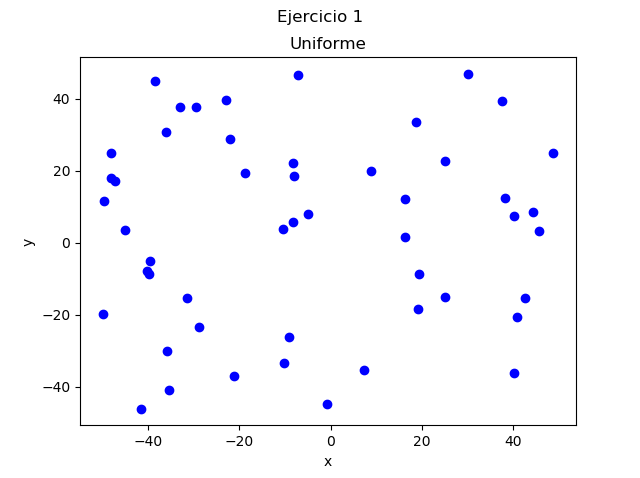
\includegraphics{images/uniforme.png}  
	\caption{Distribución uniforme de puntos en el intervalo $[-50,+50]$}
	\label{figura1}
\end{figure}

\subsubsection{Considere $N=50$, $dim=2$, $rango=[-50+50]$ con $simula_unif(N,dim,rango)$}

\begin{figure}[H]  %con el [H] le obligamos a situar aquí la figura
	\centering
	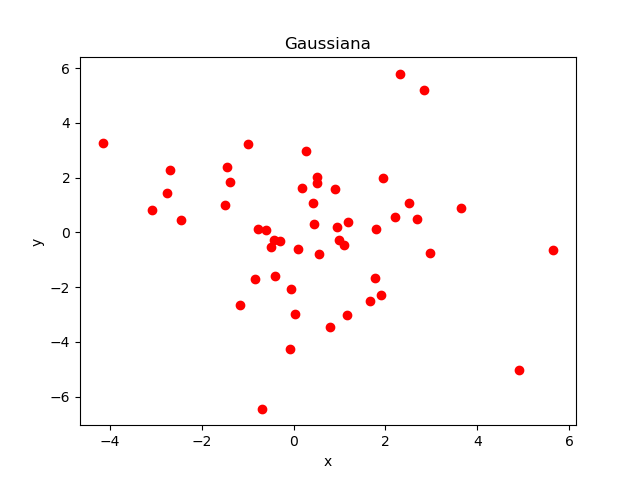
\includegraphics{images/gausiana.png}  
	\caption{Distribución gaussiana de media 0 con sigma $[5,7]$}
	\label{figura2}
\end{figure}

\subsection{Con ayuda de la función $simula_unif()$ generar una muestra de puntos 2D a los que vamos añadir una etiqueta usando la función $f(x,y)=y-ax-b$, es decir el signo de la distancia de cada punto a la recta simulada con $simula_recta()$}

\subsubsection{Dibujar una gráfica donde los puntos muestren el resultado de su etiqueta, junto con la recta usada para ello.(Observe que todos lo puntos están bien clasificados respecto de la recta.)}

\begin{figure}[H]  %con el [H] le obligamos a situar aquí la figura
	\centering
	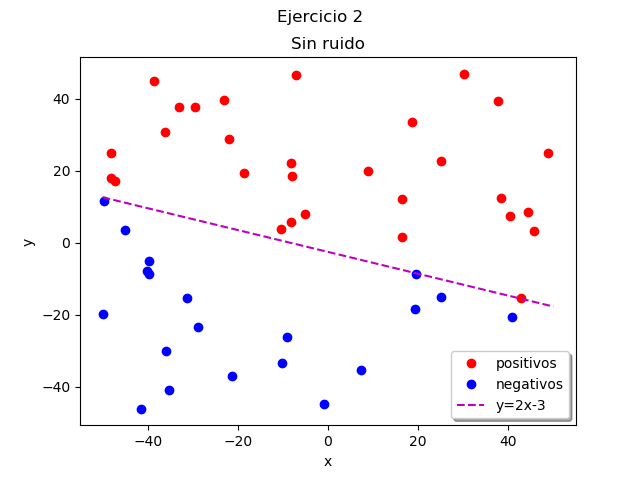
\includegraphics{images/ejercicio2Sinruido.png}  
	\caption{Puntos ``sin ruido'' clasificados con la función $f(x,y)=y-ax-b$}
	\label{figura3}
\end{figure}

\subsubsection{Modifique de forma aleatoria un $10\%$ etiquetas positivas y otro $10\%$ etiquetas negativas y guarde los puntos con sus nuevas etiquetas. Dibuje de nuevo la gráfica anterior(Ahora hay puntos mal clasificados respecto a la recta))}
\begin{figure}[H]  %con el [H] le obligamos a situar aquí la figura
	\centering
	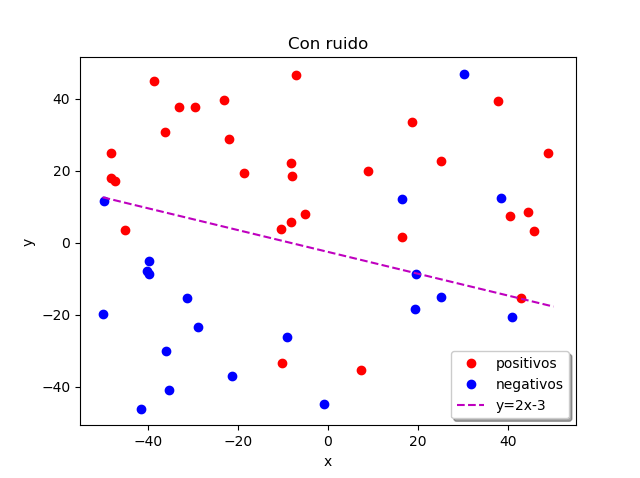
\includegraphics{images/ejercicio2ConRuido.png}  
	\caption{Puntos ``con ruido'' clasificados con la función $f(x,y)=y-ax-b$}
	\label{figura4}
\end{figure}

\subsection{Supongamos ahora que las siguientes funciones definen la frontera de clasificación de los puntos de la muestra en lugar de una recta}
\subsubsection{$f(x, y)=(x-10)^{2}+(y-20)^{2}-400$}
\begin{figure}[H]  %con el [H] le obligamos a situar aquí la figura
	\centering
	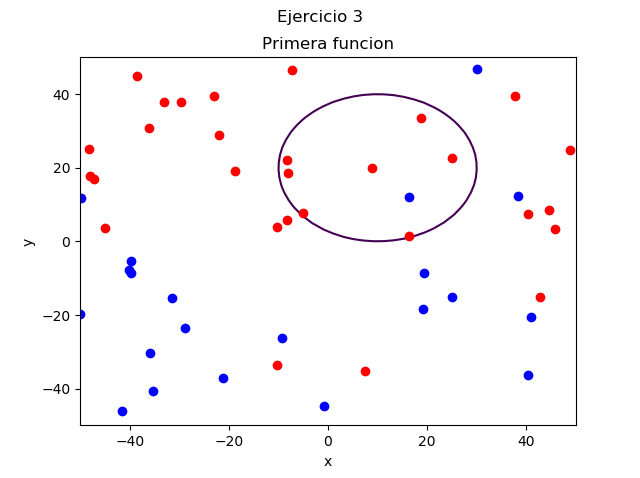
\includegraphics{images/primeraFuncion.png}  
	\caption{Primera función de frontera de clasificación}
	\label{figura5}
\end{figure}
\subsubsection{$f(x, y)=0,5(x+10)^{2}+(y-20)^{2}-400$}
\begin{figure}[H]  %con el [H] le obligamos a situar aquí la figura
	\centering
	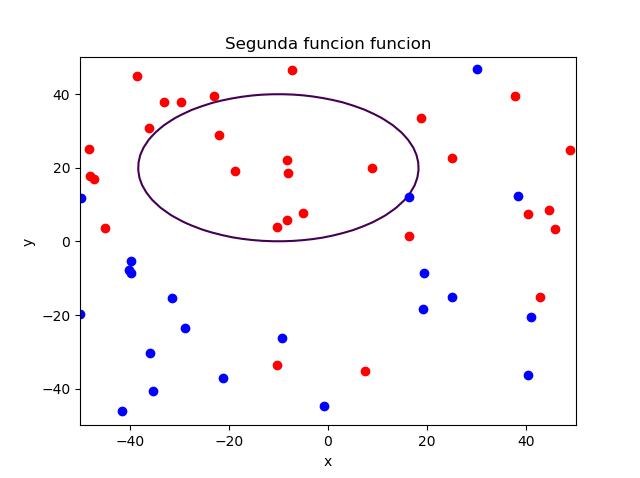
\includegraphics{images/segundafuncion.png}  
	\caption{Segunda función de frontera de clasificación}
	\label{figura6}
\end{figure}
\subsubsection{$f(x, y)=0,5(x-10)^{2}-(y+20)^{2}-400$}
\begin{figure}[H]  %con el [H] le obligamos a situar aquí la figura
	\centering
	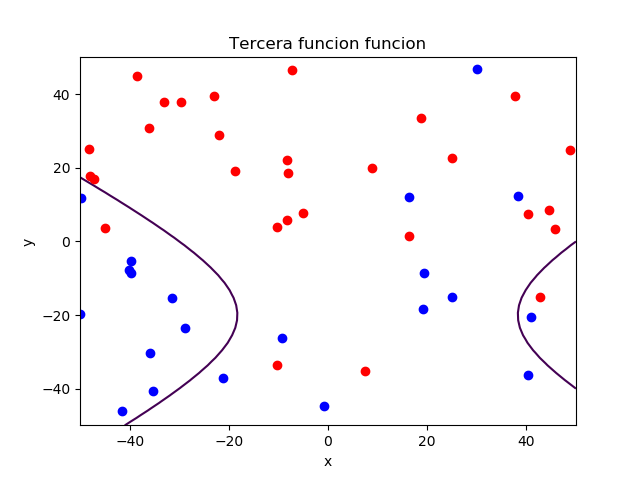
\includegraphics{images/tercerafuncion.png}  
	\caption{Tercera función de frontera de clasificación}
	\label{figura7}
\end{figure}
\subsubsection{$f(x, y)=y-20 x^{2}-5 x+3$}
\begin{figure}[H]  %con el [H] le obligamos a situar aquí la figura
	\centering
	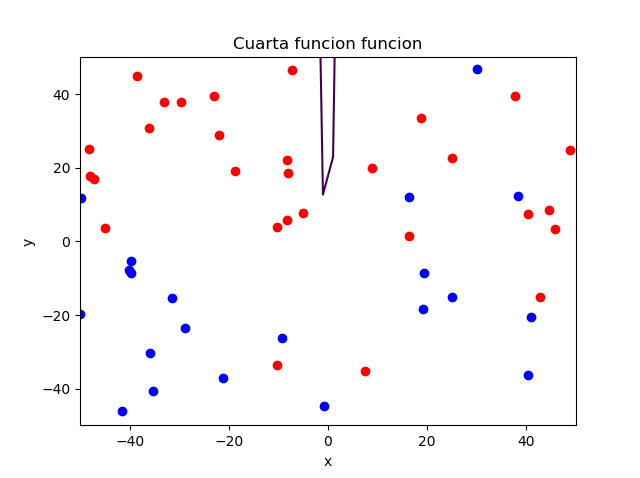
\includegraphics{images/cuartafuncion.png}  
	\caption{Cuarta función de frontera de clasificación}
	\label{figura8}
\end{figure}
\subsubsection{Análisis de las clasificaciones obtenidos}
Empezamos a analizar la primera y segunda función ya que son muy parecidas entre ellas. Podemos ver que al contrario que la recta que divide el plano en dos partes infinitas, las elipses separan para el plano en dos partes, pero una de ellas (la interior) estaría acotada. Ademas en la segunda, todo el interior estaría bien clasificado, pero en cambio ``fuera'' hay muchos mas fallos.\\
En la tercera volvemos a tener dos partes de tamaño infinito. Aunque sigue sin clasificar bien todos los puntos. En la cuarta, no clasifica bien ninguno, ya que el interior de la función no tiene ningún punto dentro. Esta tipo de funciones pueden ser buenas para otro tipos de datos(como los del ejercicio 2 de la practica anterior), pero no para los nuestros.
\section{Modelos lineales}
\subsection{Perceptron}
Debemos implementar la función $ajusta_PLA(datos,label,max_iter,vini)$ que calcula el hiperplano solución a un problema de clasificación binaria usando el algoritmo PLA. La entrada $datos$ es una matriz donde cada ítem con su etiqueta está representado por una fila de la matriz $label$ el vector de etiquetas ( cada etiqueta es un valor $+1$ o $-1$), $max_iter$ es el número máximo de iteracciones permitidas y $vini$ el valor inicial del vector. La función devuelve los coeficientes del hiperplano. El codigo de la implementación es el siguiente:\\ 
\begin{lstlisting}[language=Python]

def ajusta_PLA(datos, label, max_iter, vini):
_w = vini
_X =  np.insert(datos,0,1,axis=1)
_iteraciones = 0
_cant_cambios = 1
while _iteraciones < max_iter and _cant_cambios != 0:
	_cant_cambios = 0
	_iteraciones+= 1
	for _ix, xf in enumerate(_X):
		if np.sign(_w.T @ xf) != label[_ix]:
		_w = _w+label[_ix]*xf
		_cant_cambios += 1
return _w,_iteraciones
\end{lstlisting}
\subsubsection{Ejecutar PLA con los datos simulados en los apartado 2a de la sección 1}
El algoritmo se ejecutara con diferentes inicializaciones.
\begin{enumerate}
	\item El vector a cero
	\item Con vectores de números aleatorios en $[0,1]$ (10 veces).Anotando el número medio de iteraciones necesarias en ambos para converger. Valorar el resultado relacionando el punto de inicio con el numero de iteracciones.
\end{enumerate}
Cuando tenemos el vector inicializado a ceros, obtenemos \textbf{15 iteracciones} y cuando lo inicializo a números aleatorios obtengo una media de \textbf{9.2 iteracciones}. Por tanto tenemos que cuando el vector esta inicializado aleatoriamente necesita menos pasos, esto se puede deber a que de esta forma podemos encontrar pesos que están mas cercanos a la solución final.
\subsubsection{Ejecutar ahora PLA pero con los datos simulados en los apartado 2b de la sección 1}
En este caso, las dos veces llega al numero máximo de iteracciones, es decir \textbf{1000 iteracciones}. Esto se debe a que el perceptron no es capaz de convencer cuando hay ruido en las muestras de datos. Ya que siempre va a cambiar algún elemento y nunca a va ser capaz de recorrer todos los datos sin cambiar nada.
\subsection{Regresión logística}
En este ejercicio crearemos nuestra propia función objetivo $f$ (una probabilidad en este caso) y nuestro conjunto de datos  $\mathcal{D}$ para ver cómo funciona regresión logística. Supondremos por simplicidad que $f$ es una probabilidad con valores $0/1$ y por tanto que la etiqueta $y$ es una función determinista de \textbf{x}.\\
Consideremos $d=2$ para que los datos sean visualizables, y sea $\mathcal{X}=[0,2] \times [0,2]$ con probabilidad uniforme de elegir cada $\mathbf{x} \in \mathcal{X}$. Elegir una linea en el plano que pase por $\mathcal{X}$ como frontera entre $f(x) = 1$ (donde $y$ toma valores $+1$) y v$f(x) = 0$ (donde $y$ toma valores $-1$), para ello seleccionar dos puntos aleatorios del plano y calcular la línea que pasa por ambos. Seleccionar $N=100$ puntos aleatorios $[x_n]$ de $\mathcal{X}$ y evaluar las respuestas $\{y_n\}$ de todos ellos respecto de la frontera elegida.
\subsection{Implementar RL con SGD bajo las siguientes condiciones}
\begin{enumerate}
	\item Inicializar el vector de pesos a 0
	\item Parar el algoritmo cuando $\left\|\mathbf{w}^{(t-1)}-\mathbf{w}^{(t)}\right\|<0,01$, donde $w^{(t)}$ denota el vector de pesos al final de la época $t$. Una época es un pase completo  a través de los \textbf{N} datos.
	\item Aplicar una permutanción aleatoria $1,2,...,N$, en el orden de los datos antes de usarlos en cada epoca del algoritmo.
	\item Usar una tasa de aprendizaje de $\eta = 0,01$
\end{enumerate}
Era un código bastante largo que he evitado poner aquí. No obstante esta todo en los ficheros Python que se adjuntan con la practica.\\\\
Podemos ver como RL ajusta bien para la muestra que tenemos de 100 puntos. 
\begin{figure}[H]  %con el [H] le obligamos a situar aquí la figura
	\centering
	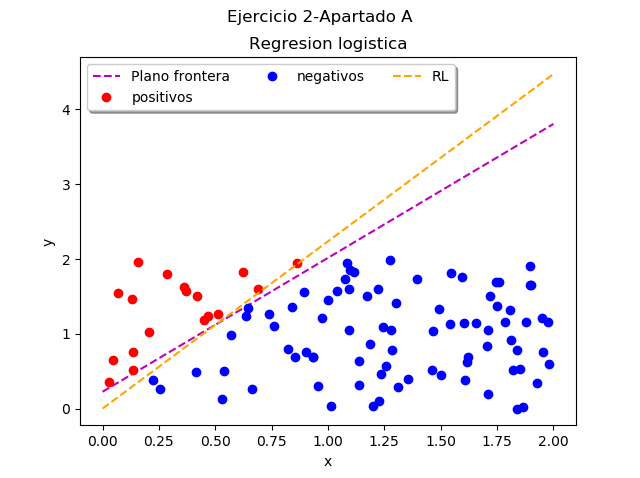
\includegraphics{images/ejercicio2ApartadoA.png}  
	\caption{100 puntos uniformes, RL y el plano frontera original}
	\label{figura9}
\end{figure}
\subsection{Usar una muestra de datos etiquetada para encontrar  nuestra solución $g$ y estimar $E_{out}$ usando para ello un número suficientemente grande de nuevas muestras $(>999)$}
Usando los mismo pesos que hemos obtenido en el apartado anterior, vamos obtener que el error va aumentar, ya que habrá puntos que se encuentre entre el plano frontera y el hiperplano que nos devuelven los pesos. 
\begin{figure}[H]  %con el [H] le obligamos a situar aquí la figura
	\centering
	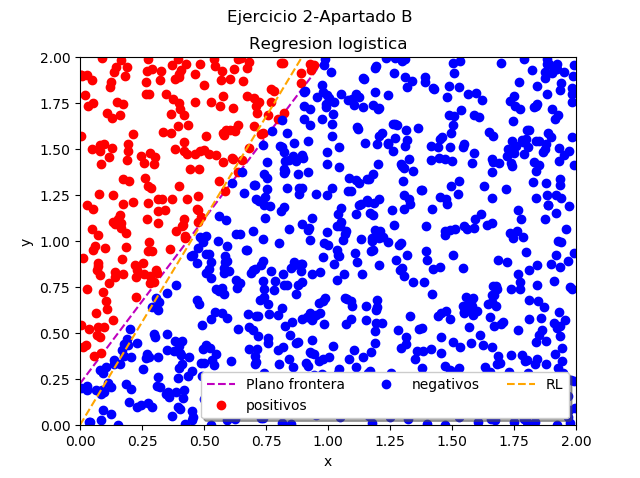
\includegraphics{images/ejercicio2ApartadoB.png}  
	\caption{1000 puntos uniformes, RL y el plano frontera original}
	\label{figura10}
\end{figure}
El $e_{out} = 0.11304005135194581$, que aun siendo bajo, ya es algo mas significativo.
\end{document}